\documentclass[11pt]{article}
\usepackage[margin=0.8in]{geometry}
\usepackage{graphicx}
\usepackage{array}
\begin{document}
\section*{Weighted common 2+2 source prefix}
The native checker matches the exact Rust statements from input destructuring through the ordered $B=0$ and $C=0$ returns. Mutation checks reject a changed cross input, determinant sign, and guard. The Lean model proves the coefficient scales $B\mapsto Z^8B$, $A\mapsto Z^9WA$, $C\mapsto Z^7WC$ under its weighted numerator equations, and characterizes the abstract branch by nonzero $B,C$.

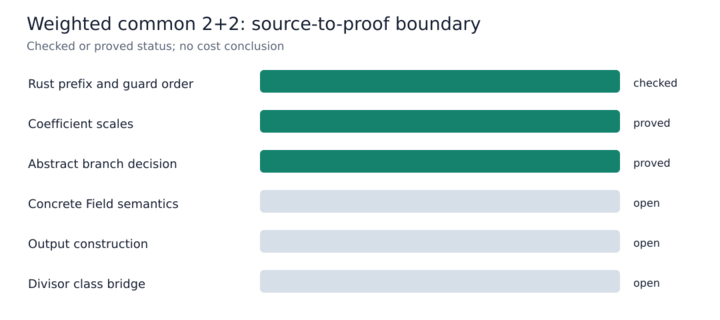
\includegraphics[width=\linewidth]{weighted-source22.png}

\noindent\textbf{Boundary.} This is a source-shape check and an algebraic theorem, not a verified compilation of Rust into Lean. Concrete \texttt{Field} semantics, output construction, and the principal-divisor/$\mathrm{Pic}^0$ bridge remain open. No cost ratio changes.

\smallskip\noindent\textbf{Reproduction.} Run the native \texttt{verify-weighted-source22} binary and compile \texttt{WeightedSource22.lean}; see the source certificate, CSV, and Lean axiom log beside this report.
\end{document}
